\section{GPU Architecture and Concepts}\label{gpu}
In this section the history of GPUs from their initial use for pixel generation in gaming to the parallel data processing titans they are today is looked at. More specifically we focus on the NVIDIA GTX 750 Ti, and how its GM107 architecture has improved to give high performance with low power consumption. The GPU programming language, CUDA, is discussed as well as CUDA best practices for optimizing the run time of the code.
%--------------------------------------------------------------------------------------
\subsection{Parallelism}\label{gpu:sec:par}
One of the main means of reducing processing time is through parallelism. The two main forms of parallelism are task and data parallelism. Task parallelism can be seen as running multiple processes concurrently where communication between the processes is explicitly defined to avoid race conditions \citep{subhlok1993exploiting}. Data parallelism is the distribution of a data set over a number of identical processes each of which performs operations on a unique subset of the data. Race conditions occur when parallel processing streams access data or perform operations out of the intended order, leading to errors or incorrect output being produced. A combination of task and data parallelism can lead to an ideal speed-up, but both have their limits depending on the task and the data being operated on \citep{subhlok1993exploiting}.
\\
\\
The increased need for parallelism came about in 2005, when \gls{cpu} frequency peaked at 4 GHz due to heat dissipation issues. However, Moore's Law \citep{moore2006cramming}, still holds, and is still expected to hold until 2025 (that is, that the number of transistors in a processor will double every two years). This leads to a problem where the speed at which an operation is done cannot be increased (due to the frequency limit), but the number of concurrent operations can still increase. This means that the only way to speed up an operation is to change it from a sequential to a parallel process \citep{rajan2013informatics}.
%--------------------------------------------------------------------------------------
\subsection{GPU Execution}\label{gpu:sec:opt}
\gls{gpu}s were originally designed for rendering pixels and vectors in games. They were especially designed for this since \gls{cpu}s are optimized to run sequential instructions as fast as possible, whereas pixel and vector calculations are inherently parallel. With NVIDIA's release of CUDA in 2006, \gls{gpgpu} programming became feasible as a way to accelerate data processing using both data and task parallelism through the simultaneous execution of similar tasks \citep{cuda_home}.
\\
\\
The power of a \gls{gpu} stems from its architecture which is optimized for a special case of \gls{simd} processing known as \gls{simt}. \gls{simd} allows a central processor to distribute a set of instructions to multiple simple processors which act on the data simultaneously. \gls{simt} is more generalized as each warp (Section \ref{gpu:ssec:smm}) of the \gls{gpu} can perform different tasks given the same set of instructions. This is due to the way in which the \gls{gpu} handles branching at the thread level. By exploiting these processes, and this instructional architecture, some instructions can be computed faster than is possible on a  a \gls{cpu} \citep{vuduc2013brief}.
%--------------------------------------------------------------------------------------
\subsection{The NVIDIA GeForce GTX 750 Ti}\label{gpu:sec:750}
%
\subsubsection{GM107 Maxwell Architecture}\label{gpu:ssec:max}
The NVIDIA GeForce GTX 750 Ti \gls{gpu} was released on the 18th of February 2014. It boasts 640 CUDA cores, 1020 MHz base clock speed, 1305.6 GFLOPs and a memory bandwidth of 86.4 GB/sec. It is NVIDIA's first-generation Maxwell architecture, designed for high performance at relatively low power consumption (60 W) and has the codename 'GM107'. The \gls{gpu} uses PCI Express 3.0 to interface with the host machine through the GigaThread engine. The first-generation Maxwell (from now simply referred to as Maxwell) is made up of one \gls{gpc} on which the processing occurs. It also contains a large L2 cache at 2048 KB and two 64-bit memory controllers to access the 2048 MB global memory. This design can be seen in Figure \ref{gpu:img:gm107} \citep{geforce_750}, \citep{g750_paper}.
%
\begin{figure}[H]
 \centering
 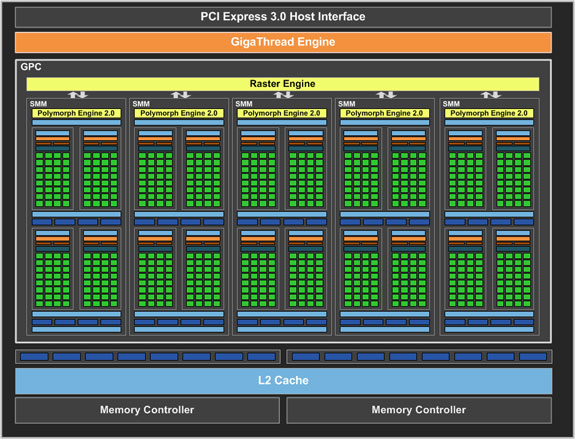
\includegraphics[width=0.5\textwidth]{Images/GM107.jpg}
 \caption[]{NVIDIA Maxwell Architecture.\footnotemark}
 \label{gpu:img:gm107}
\end{figure}
\footnotetext{Taken from \url{http://www.hitechlegion.com/reviews/graphics}}
%
\subsubsection{Streaming Multiprocessors}\label{gpu:ssec:smm}
The \gls{gpc} is further broken down into five \gls{sm}s which are divided into four processing blocks. The processing blocks (or warps) each contain an instruction buffer, a scheduler and 32 CUDA cores as seen in Figure \ref{gpu:img:smm}. These warps are set in a lock step, meaning each core in a warp executes the same set of commands at the same time, with different valued variables \citep{CUDA}.
%
\begin{figure}[H]
\centering
 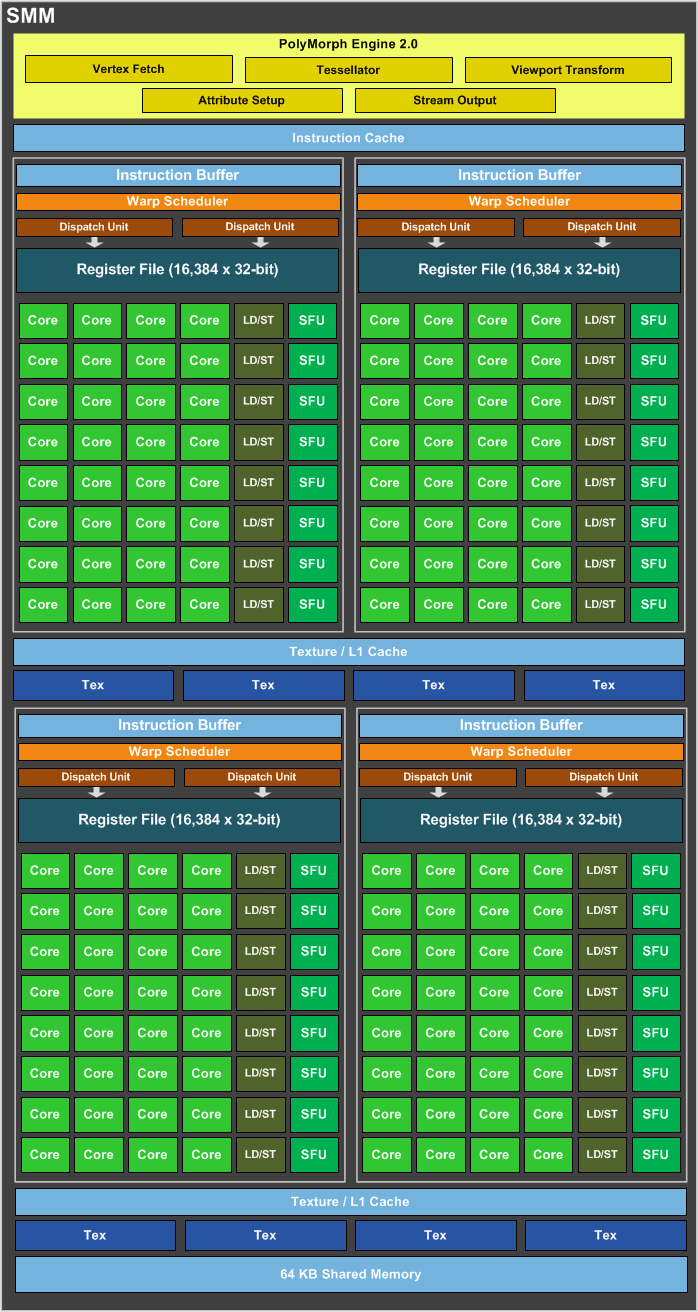
\includegraphics[width=0.3\textwidth]{Images/GM107SMM.png}
 \caption[]{Maxwell Streaming Multiprocessor.\footnotemark}
 \label{gpu:img:smm}
\end{figure}
\footnotetext{Taken from \url{http://www.legitreviews.com}}
%--------------------------------------------------------------------------------------
\subsection{CUDA}\label{gpu:sec:cuda}
CUDA is a parallel programming language created by NVIDIA for the purpose of running on their brand of \gls{gpu}s. CUDA was modelled as a C-like language with some C++ features. Its main feature is the way in which it separates \gls{cpu} and \gls{gpu} code. The \gls{cpu} code is labelled as ``host'' code and the GPU's as ``device'' code. Device code is called by the host through a special case of a method, known as a kernel. The basic structure of a kernel is as follows: 
\\
\\
\texttt{kernel0<<<grid, block>>>(params);}
\\
\\
In this instance \texttt{kernel0} would be the name of the kernel being called, \texttt{grid} is the three dimensional value of the number of blocks to be assigned, \texttt{block} being similar to \texttt{grid} is a three dimensional value of the number of threads needed and \texttt{params} is simply the parameters needed by the kernel to execute (similar to those of a method) \citep{CUDA}.
%
\subsubsection{Threads}\label{gpu:ssec:thread}
The thread is the smallest processing unit of the \gls{gpu}. \gls{gpu} threads are designed to be cheap and lightweight compared to those of a \gls{cpu} so that a thread can easily be created, run its small task and be destroyed to make place for the next thread. Threads are arranged into \gls{3d} blocks with each thread having a unique \gls{3d} ID within that block, namely an x, y and z ID. Generally the thread ID is used as the means of determining the difference in the task process of each thread \citep{CUDA}.
%
\subsubsection{Blocks}\label{gpu:ssec:block}
Each block may have a maximum of 2056 threads in total and 1024 for any single dimension; this is the reason why they are bundled into a larger, \gls{3d} grid structure. Similarly to threads, blocks have a unique \gls{3d} ID in the grid. While warps execute each step of a process simultaneously, this is not necessarily true for blocks when spread over multiple warps. More often than not, blocks exchange data within their threads and if precautions such as thread synchronisation are not taken, race conditions could ensue to break the code. Each block, when executing, must occupy a whole number of warps (rounded up). This is done as warps are constantly in lock step. Threads within a block share a fast memory, located in the L1 cache of the streaming multiprocessor. This shared memory must be preallocated when the kernel is called as a third parameter within the kernel launch (parameters within the triple angle brackets) \citep{CUDA}.
%
\subsubsection{GPU Memory Hierarchy}\label{gpu:ssec:mem}
In order to maximize concurrency on the card, the \gls{gpu} has a structured memory hierarchy. The largest, slowest and most generally accessible of these is the global memory which resides on the device memory. This memory is visible to every thread and also to every kernel called in one application. 
\\
\\
The constant memory also resides on the device memory; as the name suggests, values stored here cannot be altered and are read-only until the space is deallocated. Variables stored in constant memory also have the ability to broadcast their values to multiple threads simultaneously.
\\
\\
Similar to constant memory, texture memory also lies on the device memory and is also read-only; it is optimized for storing 2D arrays where multiple neighboring values of the array can be read concurrently.
\\
\\
The shared memory lies on the SM and is visible only to a block as a means for threads within a block to exchange data. Shared memory must be declared with the size of the memory needed (up to the maximum $64$ Kb) when the kernel is executed.
\\
\\
Each processor is assigned its own memory space to be used by each thread, in the form of registers. Registers are visible only by the thread currently on that processor and reset with each change of thread. Registers hold the variables created in and passed to the thread. The register is by far the smallest memory on the card at 32 bits per register, but 255 registers per thread. Should the thread call too many variables or variables too large to fit in the registers, the variables spill over into local memory, which lies in the L1 and L2 caches for active threads. Should the thread need to be temporarily halted for another thread to use the processor, the thread's variables are stored in local memory on the device memory \citep{CUDA}. A visual description of the memory hierarchy can be seen in Figure \ref{gpu:img:mem}.
%
\begin{figure}[H]
\centering
 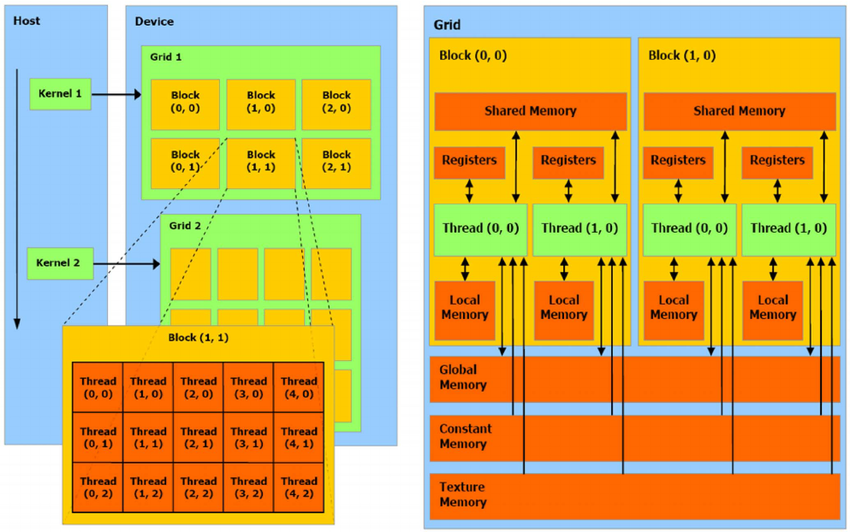
\includegraphics[width=0.7\textwidth]{Images/Cuda_mem_struct.png}
 \caption[]{CUDA memory hierarchy.\footnotemark}
 \label{gpu:img:mem}
\end{figure}
\footnotetext{Taken from \url{https://www.researchgate.net}}
%
\subsection{CUDA Optimization}\label{gpu:sec:cop}
As stated in Section \ref{gpu:sec:opt}, GPUs are designed for parallel computing to speed up the execution of a process when compared with running it on a CPU. To ensure the greatest speed-up a variety of optimizations are typically necessary to improve naive parallel code. These optimizations can be categorized into three groups, memory, execution configuration and instruction optimizations. The NVIDIA Visual Profiler (NVVP) is invaluable in assisting users to identify areas in their CUDA code that require optimization.
\subsubsection{Memory Optimization}
Memory optimization seeks to maximize the bandwidth of the GPU so that more time is spent using the faster memory (e.g. registers, L1 and L2 caches) and less time on the slower memory (e.g. device memory, host memory). An example of a memory optimization is that CUDA has the ability to asynchronously transfer data between the host and device by breaking a kernel into streams, thereby allowing the device to process one section of the data while another is still being transferred to it and a third is being transferred back to the host. Alternately, memory on the host can simply be mapped to the device. This memory is accessible by both the host and device and is known as zero-copy memory. This can only be done on pinned memory, which is memory set aside by CUDA to be used by the GPU, and is also optimized to have a higher transfer rate to the GPU than any other host memory. This can be taken a step further through unified virtual addressing, where the host and device share a single virtual memory space; this address space lies on the host, but through predictions by CUDA on the need for certain sections of the memory, parts of the memory are transferred to the device as they are needed. The different types of memory found in the GPU as discussed in Section \ref{gpu:ssec:mem} show examples of this as well. Constant and texture memory, for example, improve latency by having the value broadcast to all threads and 2D spatial locality read abilities, respectively. The use of sequential reads and stride accessing can also improve bandwidth usage as the memory required is aligned on the device \citep{CUDA}.
%
\subsubsection{Execution Configuration Optimization}
Execution configuration optimizations seek to improve the overall usage of cores on the GPU, keeping as much of the hardware as possible occupied to improve the overall execution time. One way of achieving this is through concurrent kernel execution, that is, multiple kernels running concurrently to reduce the idle time of each warp. Another way is by setting the number of threads in a block to always be a multiple of 32 so that all the cores in a warp are occupied. Other examples include having multiple small blocks instead of a single large block, especially when using thread synchronizations and also having a minimum block size of 32 threads \citep{CUDA}.
%
\subsubsection{Instruction Optimization}
Instruction optimization uses the knowledge of how certain instructions are executed to speed up code in critical areas. This form of optimization is most prevalent in arithmetic operations. Most notably, single precision is encouraged as well as using the multiple CUDA maths libraries that interface directly with the hardware. These libraries include cuBLAS for linear algebra, cuSparse for sparse matrix operations, cuRAND for random number generation, nvGRAPH for graph analytics and cuFFT for fast Fourier transforms. These and more libraries are discussed in \citep{CUDA_lib}. Another way of reducing latency is by minimizing the use of global memory, as it is generally the slowest to access. Making use of constant and shared memory for read-only values and shared memory for block specific values can drastically improve memory access times \citep{CUDA}.
%--------------------------------------------------------------------------------------
\subsection{Related Work}\label{gpu:sec:rel}
Only one study relating to GPU implementation of a Voronoi tessellation has, to the best of our knowledge, been published. This algorithm is called "Jump Flooding" and is explained below.
\\
\\
\citet{rong2006jump} describe a method of approximating a Voronoi transform using a method known as jump flooding. The algorithm works by seeing the space as a discrete $n \times n$ grid. It works by having grid cells with an identified closest seed point (or in this case, seed cell) and projecting this seed cell to surrounding cells without an identified seed cell in incrementally smaller steps, starting from a step size of $n/2$.
\\
\\
While the Jump Flood does outperform standard CPU algorithms, it is sensitive to the resolution of the output grid. Therefore the algorithm could potentially be slower than a CPU implementation where the CPU implementation is grid independent, such as the divide and conquer or Fortune's algorithm.
%--------------------------------------------------------------------------------------